\section{Introduction}
\label{sec:introduction}
Lightyear designs and develops solar electric vehicles (SEVs), these are highly efficient battery electric vehicles that can charge their batteries using an integrated solar panel. The following factors play a role in a vehicle's efficiency: Aerodynamic drag, friction losses from tires, cabin heating and cooling, drivetrain losses, static energy consumption. Lightyear seeks to design a vehicle that minimizes these losses as a reduction in energy consumption has a snowball effect on vehicle efficiency. For example, a lower aerodynamic drag enables the use of a smaller battery pack while maintaining the same range, reducing the vehicle weight, resulting in less friction losses from the tires etc. In the end yielding a very efficient vehicle.

\subsection{Current and future automotive architectures}
\label{sec:automotive-arch}
Modern vehicles are mostly electrically/electronically controlled, ranging from basic functionality such as acceleration (throttle pedal) and lighting to more advanced features such as ride height control and Autonomous Emergency Braking System. The number of electrically/electronically controlled features has grown over time by adding several electronic control units (ECUs) per feature to an already existing decentralized control architecture. This means that multiple ECUs need to communicate in order to achieve a certain function. As a result modern vehicles can contain more than 100 ECUs~\cite{bandur2021making} and several communication networks. This has several drawbacks: increased communication load on the in-vehicle network(s), increased cost due to the large number of ECUs and large wiring harness, increased software complexity, more software variants, higher maintenance costs and reduced reliability~\cite{bandur2021making}. An example of such a decentralized architecture is shown in Figure~\ref{fig:functional-arch}, the blue rectangles represent ECUs, ECUs that are part of a single function or domain (body control, drivetrain etc) are connected to each other with an automotive network such as LIN or CAN. The functions or domains work together by means of a gateway (red rectangle) which bridges or translates messages to and from the different networks. Sometimes certain ECUs are also connected to more than one network for practical reasons such as the Steering column ECU in the example.

\begin{figure}[htb]
    \centering
    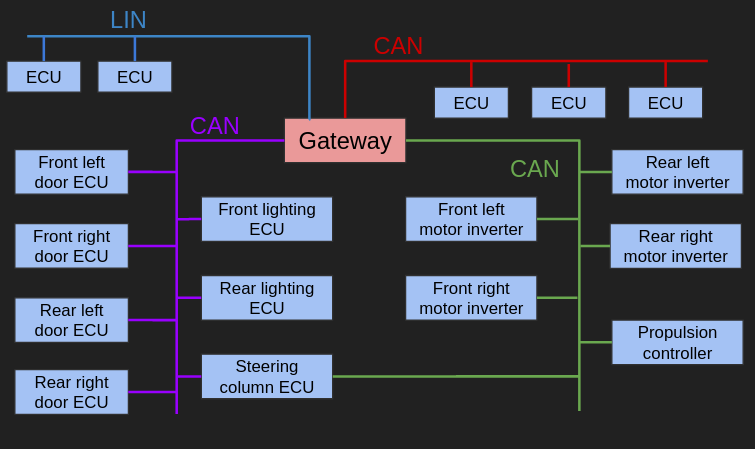
\includegraphics[width=\textwidth]{images/functional-arch.png}
    \caption{Example of an automotive decentralized control architecture}
    \label{fig:functional-arch}
\end{figure}

The automotive industry has recognized these issues and is moving towards a centralized control architecture with one large ECU per physical zone, called a zonal architecture~\cite{ashjaei2021time}. Instead of having many small ECUs performing only one part of a function there will be one central ECU responsible for all the control functions and a few large ECUs (zone ECUs) strategically placed in the car executing the commands of the central controller. To reduce complexity, weight and cost even more the zone ECUs are networked through a single high bandwidth, low latency network instead of the multiple low bandwidth networks running through a vehicle nowadays. The zone ECUs can act as a bridge for legacy networks used by legacy components in the physical neighbourhood. An example is depicted in Figure~\ref{fig:zonal-arch}.

In the zonal architecture the zone ECUs and central controller are connected through a high bandwidth low latency network, automotive Ethernet together with Time Sensitive Networking (TSN) have been chosen as the key networking technologies. The choice for automotive Ethernet is supported by the work of the Time Sensitive Networking (TSN) Task Group of the IEEE 802.1 Working Group, which allow real-time communication over IEEE 802.3 (Ethernet) networks~\cite{klaus2019zonal}. Other relevant factors are the high bandwidth capabilities relative to traditional networking technologies such as CAN and FlexRay, Internet Protocol (IP) based end to end communication support, automotive specific physical layer standards for various data rates and standardization by the IEEE~\cite{ashjaei2021time}.

Figure~\ref{fig:zonal-arch} represents the same vehicle as in Figure~\ref{fig:functional-arch} with a zonal architecture. The number of ECUs, including gateway, is reduced from 18 in the decentralized architecture to 11 in the zonal architecture. This reduction has been achieved by consolidating several ECUs into the zone ECUs, reducing mass. The number of networks has stayed the same, three CAN networks and one LIN network in the decentralized control architecture versus 3 CAN networks and one Ethernet network in the zonal architecture. But crucially the physical wiring loom has been simplified in the zonal architecture as there is only one network cable spanning the entire vehicle length. This simplification reduces weight, since there is only one cable going from the back to the front instead of two or more. Additionally, the shorter sub-wire harnesses can be manufactured automatically, reducing costs.

\begin{figure}[htb]
    \centering
    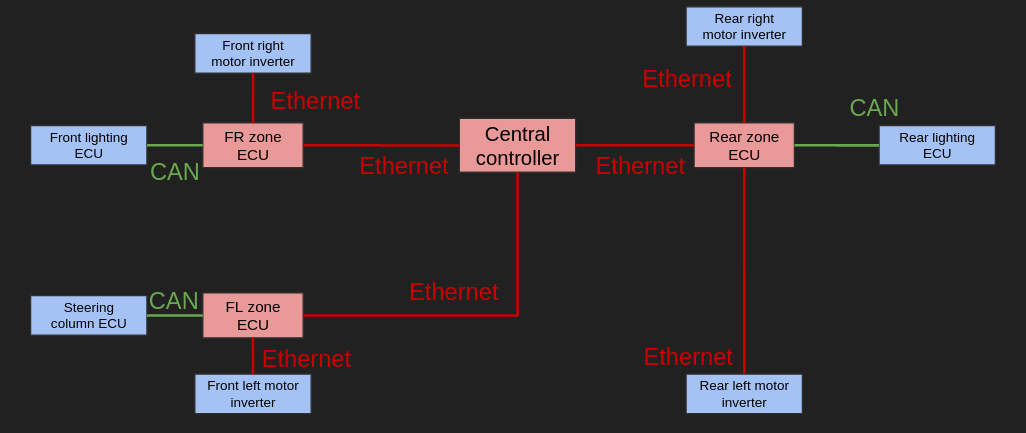
\includegraphics[width=\textwidth]{images/zone-arch.png}
    \caption{Example of an automotive zonal architecture}
    \label{fig:zonal-arch}
\end{figure}

\subsection{Real-time communication over Ethernet}
Some electrically/electronically features in a vehicle pose strict timing requirements on the architecture and implementation. For example the passenger safety system must always deploy the airbags within a specific time period after a crash. Deploying the airbags too quickly or too late can cause harm to the passengers. Systems with strict timing guarantees are called real-time systems and require the timing properties of the system to be bounded and analysable. If the implementation of such a feature requires several networked ECUs to work together the network and the ECUs should be real-time. Examples of automotive networks that support real-time communication are LIN, CAN and FlexRay. 

IEEE 802.3 Ethernet is not a real-time network, one of the original design philosophies is best-effort transmission of frames~\cite{metcalfe1976ethernet}. The idea being that it would be not economically viable to create a network that guarantees error-free message delivery. Putting the responsibility of dealing with the various possible errors, such as packet loss, duplication, large delays etc, on the communicating processes. This allows giving good average-case performance to a large group of users in an economically viable way, but sacrifices the real-time property. 

Originally Ethernet was designed as a bus network with CSMA/CD to allow multiple hosts to use a shared medium. CSMA/CD is also used as a Medium Access Control method in "modern" twisted-pair Ethernet networks where multiple nodes are in the same collision domain, for example when using half-duplex communication or when repeater hubs are used to interconnect Ethernet segments. CSMA/CD violates the real-time property because it uses a randomized exponential backoff algorithm when retransmission of frames is necessary due to simultaneous transmission by distinct nodes in the collision domain. This means that frames can be delayed a random amount of time. How often a message is delayed increases as the network load increases.

Full-duplex switched Ethernet no longer uses CSMA/CD, but the switches introduce a delay as well. IEEE 802.3 does not specify how a switch should operate, hence no guarantee can be made about the queuing and switching delay added to the transmission time by a switch. Lastly, it is reasonable to assume that queuing delays increase as the number of packets passing through a switch increases. Together this makes Ethernet unsuitable for use in a real-time system. 

Several higher level protocols have been proposed to make real-time communication on top of Ethernet possible e.g. EtherCAT, PROFINET, TTEthernet and Time Sensitive Networking. Some of these protocols require special network interface cards or switches to operate, or they are not directly interoperable with \textit{standard} Ethernet which complicates mixing the network with other devices such as a computer using the TCP/IP stack. As mentioned in Section~\ref{sec:automotive-arch}, Time Sensitive Networking (TSN) is a set of standards created by the IEEE specifically to allow interoperability on standard Ethernet networks such that real-time and non-real-time traffic can coexist on the same network.


\vfill